\documentclass[journal=jacsat,manuscript=article]{achemso}

% Image-related packages
\usepackage{graphicx}
\usepackage{subcaption}
\usepackage[export]{adjustbox}
\usepackage{wrapfig}

\newcommand*\mycommand[1]{\texttt{\emph{#1}}}

\author{Nayanika Das}
\affiliation[UVicUCC]{Computational Biochemistry and Biophysics Lab, Research Group on Bioinformatics and Bioimaging (BI$^2$), Department of Biosciences, Universitat de Vic - Universitat Central de Catalunya, 08500 Vic, Spain}
\author{Vijay Baladhye}
\affiliation[SPPU]{Savitribai Phule Punr University, Pune, India}
\author{Jordi Villà-Freixa}
\email{jordi.villa@uvic.cat}
\affiliation[UVicUCC]{Computational Biochemistry and Biophysics Lab, Research Group on Bioinformatics and Bioimaging (BI$^2$), Department of Biosciences, Universitat de Vic - Universitat Central de Catalunya, 08500 Vic, Spain}
\alsoaffiliation{IRIS-CC}

\title[Computational analysis of GPX6 activation free energy]
  {Computational analysis of the evolution of glutathione peroxidase 6 (GPX6) activation free energy}

\abbreviations{IR,NMR,UV}
\keywords{Ancestral enzyme reconstruction, enzyme design, empirical valence bond, free energy calculations}

\begin{document}

\begin{abstract}
Outstanding success in computational protein design has been achieved in recent years by combining machine learning approaches with physicochemical properties analysis of the explored variants. Despite these efforts, however, less success has been obtained in designing good computational protocols for optimization of enzyme activity. Here we propose the use of the Empirical Valence Bond method to evaluate free energies of activation of enzyme variants to obtain reasonable mutational pathways leading to a functionally optimized protein. In particular, we propose a method that explores a lower free energy difference pathway for the directed evolution of enzymes based on EVB activation free energies. To test the idea, we study the hypothetical connectivity of the selenocysteine-containing human glutathione peroxidase 6 protein (GPX6) into its ortholog cysteine-containing mouse GPX6. We show how it is possible to find a mutational pathway connecting the two protein sequences and structures that provide the empirical barriers for the first step of the GPX6-catalyzed reaction. Moreover, this protocol offers the potential for addressing complex issues such as epistasis in enzyme engineering, further enhancing its utility in enzyme optimization.
\end{abstract}

\section{Introduction}

Selenium (Se), in the form of selenocysteine (Sec, U—the 21st amino acid) occurs in 25 proteins in the human proteome. Insertion of Sec into a protein is much more complicated than the other 20 amino acids because a UGA stop codon must be recoded as a sense codon for Sec \cite{Hondal2011}. The complexity of this process signifies that Sec must fulfill a chemical function that exerts biological pressure on the genome to maintain the Sec-insertion machinery \cite{Cardey2007, Hondal2011}. Sec has unique properties such as a lower pKa and higher nucleophilicity compared to cysteine, enhancing the enzyme's catalytic properties \cite{Hondal2011, Rees2024}. Although the catalytic triad of glutathione peroxidase (GPX) has been well recognized, there has been little evidence for the relevance of the interactions among the triad amino acid, i.e., selenocysteine (U), glutamine (Q), and tryptophan (W). 

\subsection{Mechanism of GPX}

A catalytic mechanism proposed for GPX3 by Morokuma et al. involves the formation of a selenolate anion, followed by bond cleavage in hydrogen peroxide leading to the formation of selenenic acid, with a computed barrier of 18.0 kcal/mol \cite{Prabhakar2006}. Flohe et al. propose an alternate mechanism involving charge separation steps \cite{Orian2015}.

\begin{figure}[h]
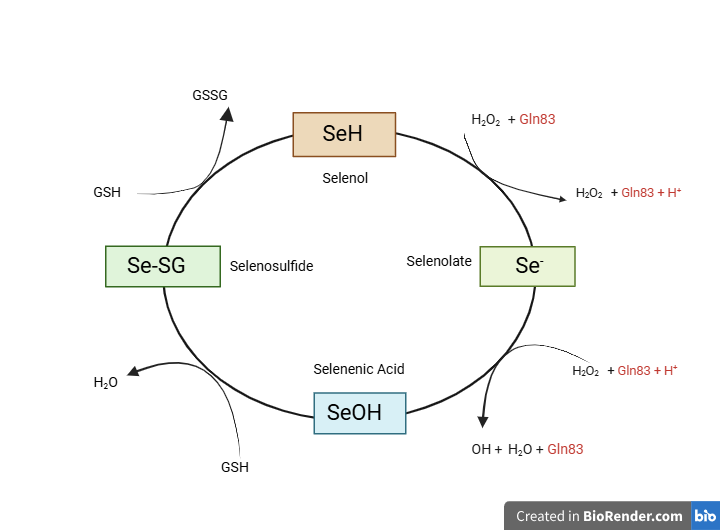
\includegraphics[width=0.7\textwidth]{figures/Catalytic_cycle.png}
\caption{Catalytic Cycle of GPX as given by Morokuma et al. where the resting state of selenium is Selenol}
\label{fig:figure1}
\end{figure}

\subsection{Empirical Valence Bond Model based on QM/MM Calculations}

The EVB approach constructs potential energy surfaces for elementary chemical reaction steps \cite{Oanca2024}. Using a two-state model, the EVB Hamiltonian provides insights into thermodynamic activation parameters based on classical force fields and coupling terms derived from DFT or QM/MM calibrations \cite{Oanca2023}.

\subsection{Directed Evolution and Epistasis in Enzyme Design}

Directed evolution mimics natural selection to optimize enzyme traits. Computational design adapts these principles to predict mutation pathways, potentially enhancing enzyme catalytic performance. By exploring mutational pathways with EVB, we investigate the activation energy variations in GPX6 homologs to assess catalytic activity changes due to selenocysteine/cysteine substitution \cite{Starr2016, Storz2018}.

\section{Computational Methodology}

The initial structure was obtained from an MD simulation snapshot. Selenium parameters were generated using FFLD in Maestro, with protonation states predicted by PROPKA \cite{Søndergaard2011}. TIP3P water was used around the protein, and after equilibration, MD/EVB free energy perturbation (FEP) calculations were done for both reaction steps, replicated over 10 iterations. The EVB parameters were calibrated based on QM/MM barriers previously calculated.

\begin{figure}
\begin{center}
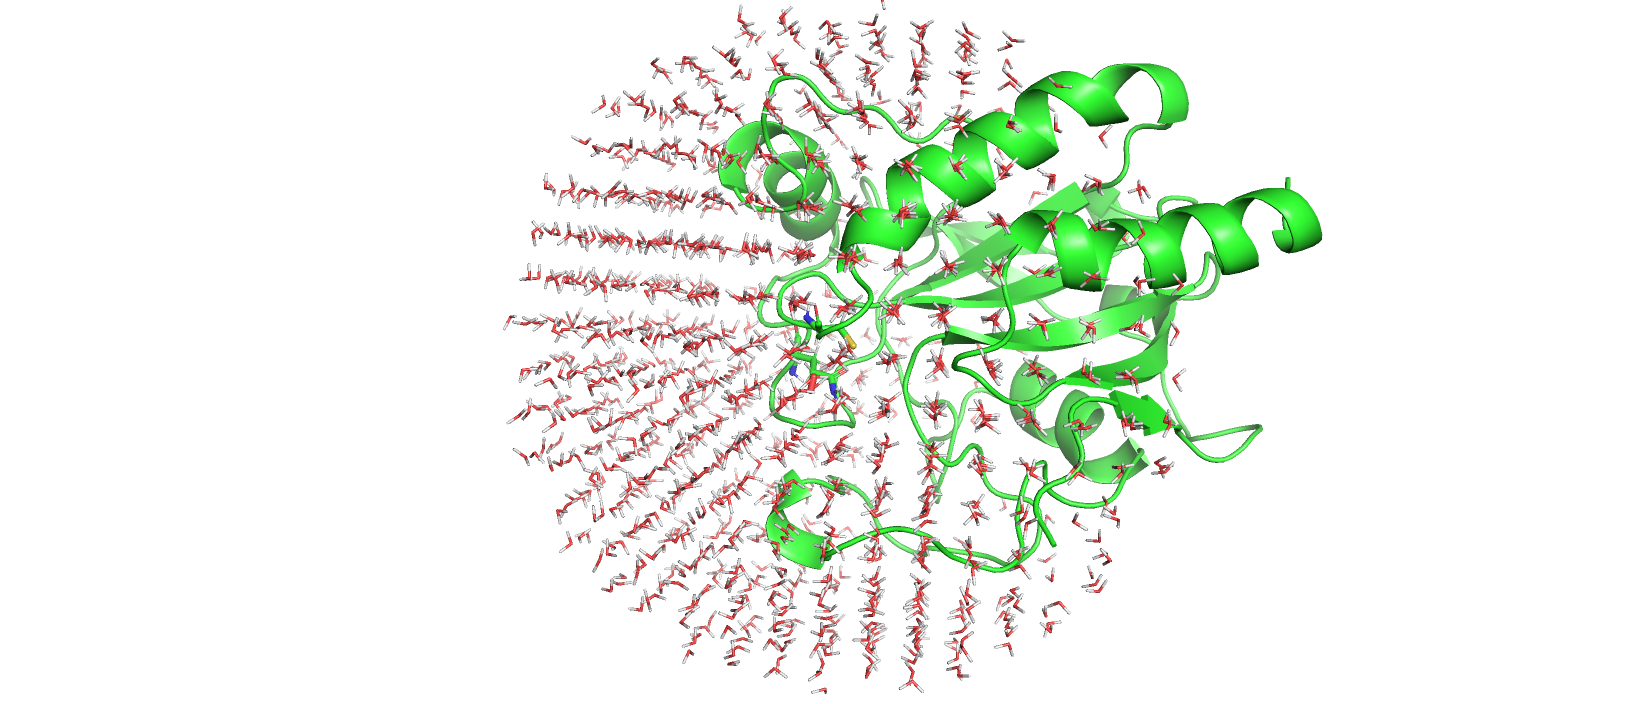
\includegraphics[width=0.7\linewidth, height=5cm]{figures/solvent_sphere.png} 
\end{center}
\caption{Sphere of water molecules around the protein}
\label{fig:figure6}
\end{figure}

\medskip

\bibliographystyle{unsrt}
\bibliography{files/references}

\end{document}
